%!TEX TS-program = xelatex
\documentclass[12pt, a4paper, oneside]{article}

\input{preamble.tex}

\begin{document}

\section*{Quiz 1: нейросеть --- всего лишь функция}

\epigraph{Нам не победить, но мы вступим с ним в битву всё равно.}{\textit{Теоден Роханский (Властелин колец: Братсво Кольца, 2001)}}

Решите все задания. Все ответы должны быть обоснованы. Решения должны быть прописаны для каждого пункта. Рисунки должны быть чёткими и понятными. Все линии должны быть подписаны. При решении работы можно пользоваться чем угодно.

\vspace{-0.5cm}
\subsection*{[3] Задание 1} 
\vspace{-0.5cm}

Любитель нейросетей Яроslave собрал полносвязную нейросеть для классификации на $3$ (три) класса с картинки \ref{pic1:yarnn}. Какие классы спрогнозирует его нейросеть для входов $x_1 = -2, x_2 = 1, x_3 = 0$? 

\vspace{-0.5cm}
% \vspace{2.5cm}
\subsection*{[4] Задание 2}
\vspace{-0.5cm}

Какие минимальное количество нейронов нужно, чтобы решить задачу классификации с картинки \ref{pic2:clf}? Объясните свой ответ и нарисуйте соответствующую архитектуру. 

% \vfill

\begin{minipage}{0.45\linewidth} 
\begin{figure}[H]
\caption{нейросеть Яроslavа}  \label{pic1:yarnn}
    \begin{center}
    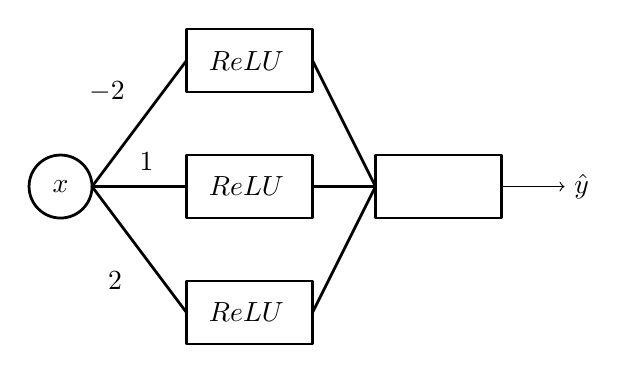
\begin{tikzpicture}[scale = 0.8, line cap=round,line join=round,x=1.0cm,y=1.0cm]
    
    \draw [line width=1.pt] (-3,0.5) circle (0.5cm) node {$x$};
    
    \draw [line width=1.pt] (-1,2)--(1,2)--(1,3)--(-1,3)--cycle;
    \draw (-0.8,2.5) node[right] {$ReLU$};
    
    \draw [line width=1.pt] (-1,0)--(1,0)--(1,1)--(-1,1)--cycle;
    \draw (-0.8,0.5) node[right] {$ReLU$};
    
    \draw [line width=1.pt] (-1,-2)--(1,-2)--(1,-1)--(-1,-1)--cycle;
    \draw (-0.8,-1.5) node[right] {$ReLU$};
    
    \draw [line width=1.pt] (-2.5,0.5) -- (-1,0.5);
    \draw (-2.7, 2) node[right] {$-2$};
    \draw [line width=1.pt] (-2.5,0.5) -- (-1,2.5);
    \draw (-1.9, 0.9) node[right] {$1$};
    \draw [line width=1.pt] (-2.5,0.5) -- (-1,-1.5);
    \draw (-2.4, -1) node[right] {$2$};
    
    \draw [line width=1.pt] (2,0)--(4,0)--(4,1)--(2,1)--cycle;
    \draw (2.0,0.5) node[right] {$\softmax$};
    
    \draw [line width=1.pt] (1,0.5) -- (2, 0.5);
    \draw [line width=1.pt] (1,2.5) -- (2, 0.5);
    \draw [line width=1.pt] (1,-1.5) -- (2, 0.5);
    
    \draw [->] (4,0.5) -- (5,0.5) node[right] {$\hat y$};
    \end{tikzpicture}
    \end{center}
\end{figure}
\end{minipage} 
\hfill
\begin{minipage}{0.45\linewidth} 
\begin{figure}[H] 
\caption{задача классификации} \label{pic2:clf}
    \begin{center}
    \begin{tikzpicture}[scale = 0.7, line cap=round,line join=round,x=1.0cm,y=1.0cm]
        \draw [->] (-2,0.5)--(3,0.5);
        \draw (3, 0.5) node[right] {$x$};
        \draw [->] (0.5,-2)--(0.5,3);
        \draw (0.5, 3) node[right] {$y$};
        
    	\draw [fill=blue] (1,2) circle (2.5pt);
    	\draw [fill=blue] (2,1) circle (2.5pt);
    	\draw [fill=blue] (2,2) circle (2.5pt);
    	
    	\draw [fill=blue] (0,-1) circle (2.5pt);
    	\draw [fill=blue] (0,0) circle (2.5pt);
    	\draw [fill=blue] (-0.5,-0.5) circle (2.5pt);
    	\draw [fill=blue] (-1,-1) circle (2.5pt);
    	\draw [fill=blue] (-1,0) circle (2.5pt);
    	
    	\path (0,1) pic[red] {cross=2.5pt};
    	\path (-1,1) pic[red] {cross=2.5pt};
    	\path (-0.5,2) pic[red] {cross=2.5pt};
    	
    	\path (1.2,0) pic[red] {cross=2.5pt};
    	\path (1,-0.5) pic[red] {cross=2.5pt};	
    	\path (2.1,0) pic[red] {cross=2.5pt};
    	\path (2,-1.3) pic[red] {cross=2.5pt};
    \end{tikzpicture}
    \end{center}
\end{figure}
\end{minipage} 

\vspace{-0.5cm}
\subsection*{[3] Задание 3}
\vspace{-0.5cm}

Машинлёрнерша Амалия написала на бумажке функцию \eqref{eq:amalia}. Нарисуйте нейронную сеть, которая соответствует этой функции. \begin{multline} \label{eq:amalia}
    y =  \max(0, 0.2 \cdot \max(0, \max(0, 0.5 \cdot x_1))) + \\ + 0.8 \cdot \max(0, 4\cdot x_2 + 2 \cdot \max(0, 0.5 \cdot x_1)) + \\ + 0.5 \cdot \max(0, 17 \cdot x_2 + 15 ) + 3)
\end{multline}  

% \vspace{6cm}
\vspace{-0.5cm}
\subsection*{[0.1] Задание 4}
\vspace{-0.5cm}

Расскажите какой именно подарок вы просили на Новый год у Деда Мороза.


\end{document}